\documentclass[12pt]{article}
\usepackage{graphicx}
\usepackage{graphicx}
\usepackage{subcaption}
\usepackage{amsmath}
\usepackage{amssymb}
	\addtolength{\oddsidemargin}{-.5in}
	\addtolength{\evensidemargin}{-.5in}
	\addtolength{\textwidth}{.5in}

	\addtolength{\topmargin}{-.5in}
	\addtolength{\textheight}{.5in}
\usepackage{fullpage}
\pagenumbering{gobble}
\begin{document}

\title{Online EM Project\\ Statistics 221
}
\author{Hannah Director, Kevin Eskici, Willy Xiao}

\maketitle

\section{Literature Review}
The \textbf{\it{Online Em Algorithm for Latent Data Models}} proposed by Cappe and Moulines seeks to define a more efficient EM algorithm for latent data models by allowing for updates that use only data from the current iteration rather than from the entire data set. For big data problems, this is highly beneficial, since storing and retrieving all the data in these types of problems is not computationally feasible. As in traditional EM, the goal of online EM remains to find the maximum likelihood estimates for a given model when the intractability of the integrals renders direct calculation of these estimates impossible. This approach is often needed because of latent variables. In this paper, Cappe and Moulines focus on this use of EM for latent variables and extend it for online use.\\

We now lay out their approach. Like in batch EM, the maximum likelihood estimates for the parameters are obtained by iterating between the E-step and the M-step. In the E-step, the expectation of the log-likelihood with respect to the latent variables given the data is found keeping the estimates of the parameters from the previous iteration as constant. In the M-step, the values of the parameters are found such that they maximize this expectation, referred to as $Q(\theta | \theta^{(t)})$. In the proposed online approach, the M-step is unchanged, but the E-step is replaced by a a stochastic approximation step. Specifically, the authors use the form of the stochastic gradient descent (sgd) for updates on $Q(\theta | \theta^{(t)})$, giving
\begin{equation}
\hat{Q}_{n+1}(\theta) = \hat{Q}_{n}(\theta) + \gamma_{n+1}(\mathbb{E}_{\hat{\theta}_{n}}[log f(X_{n+1};\theta)|Y_{n+1}] - \hat{Q}_{n}(\theta))
\end{equation}
where $\gamma_{n+1}$ corresponds to the learning rate. Assuming the complete data likelihood is from the exponential family and that there is a unique global maximum of the parameters which is a function of the sufficient statistics, $\overline{\theta}(s)$,  as well as some other regularity conditions, the E-step reduces to just finding the expectations of the complete data sufficient statistics using these sgd updates. Then the entire online EM algorithm can be summarized quite simply as follows
\begin{align}
\hat{s}_{n+1} &= \hat{s}_{n} + \gamma_{n+1}(\overline{s}(Y_{n+1}; \hat{\theta}_{n}) - \hat{s}_{n}) \nonumber \\
\hat{\theta}_{n+1} &= \overline{\theta}(\hat{s}_{n+1})
\end{align}
These steps are repeated for each $Y_{i}$ until all the data has been cycled through.\\

The theoretical justification of this approach is largely dependent on the work of Lange (1995). Lange had the insight that the M-step in batch EM can be replaced by a Newton-Raphson step or a stochastic approximation of the Newton steps (under some conditions) giving a recursion for the parameter updates that is "locally equivalent to the EM algorithm at convergence." The corresponding proposed updates are referred to as the online gradient algorithm. Cappe and Mouline show that their online updates can be manipulated to be of the same form as the online gradient algorithm when approaching convergence, so their algorithm has similar convergence performance. 




\section{Tasks}
\subsection{Implementation 1}
In this section, we implement the model for the Poisson mixture model of section 2.4. We largely follow the algorithm directly as given in the paper. It's unspecified in the paper, so we selected a learning rate of $1/2i$. We ran this model on a number of different combinations of $\lambda$, $M$, and $w$ values. We list here several examples, including a trivial case that demonstrates unit testing. \\

\noindent \underline{\textbf{Example 1: Trivial Unit Testing (M = 1)} }\\ 
\indent Simulated Model: $\lambda$  = 100, $w = 1$, 100,000 data points\\
\indent Estimated Parameters: $ \hat{\lambda} = 99.9998, \hat{w} =  1.0$\\

\noindent \underline{\textbf{Example 2: M =3 }}\\
\indent Simulated Model: $\lambda = (2, 15, 30), w = (0.5, 0.3, 0.2)$\\
\indent Estimated Parameters: $\hat{\lambda} = (2.0015, 14.9150, 29.9196), \hat{w} = (0.5003, 0.2964, 0.2032)$ \\

\noindent \underline{\textbf{Example 3: M = 2}}|\\
\indent Simulated Model: $\lambda = (10,2), w = (0.75, 0.25)$\\
\indent Estimated Parameters: $\hat{\lambda} = (10.0612, 2.0845), \hat{w} = ( 0.7424, 0.2575) $ \\

\noindent Like most models to determine underlying mixture models, this method performs well when there is a lot of seperation between the means and performs poorly when the means are quite similar. Because the method is online, this method also tends to break down if there is one  distribution with a very large or very small mean that has relatively low weight. In those cases, if one of these exteme values does not occur early on, the means of each of the mixtures starts to be set at less extreme values. Then,when an extreme value occurs, the probability of such a value occuring is numerically zero. This causes the existing algorithm to fail. 

\subsection{Implementation 2}
In this section, we implement the online EM algorithm for a mixture of Gaussian regressions. Figures 1-4 are our replications of Figures 1-4 in the paper. In implementing the Gaussian regression  algorithm, we were able to follow the method in Cappe and Moulines' paper closely, with a few exceptions. Most notably, in the paper, the update for $\overline{s}_{3,j}(r,z;\theta) = \overline{w}_{j}(r,z;\theta)rzz^{T}$; however, this is incorrect, we should update $\overline{s}_{3,j}(r,z;\theta) = \overline{w}_{j}(r,z;\theta)zz^{T}$. This is likely just a typo in the published paper, but it's problematic, since failure to notice this error results in an algorithm that does not converge. Additionally, how to  initialize $M_{j}$, the ($d_{z} + 1)$-dimension matrix block that defines the sufficient statistics, is not specified in the paper. We chose to make $4 \times 4$ random matrices for each j, then set $M = A^{T}A$ for the first iteration. Lastly, the paper does not give any details on how the batch EM implementation is run. We assumed that they used a straightforward implementation, since batch EM was included only as a point of comparison. Correspondingly, we found the Batch EM values using the simple implementation provided by \textit{regmixEM} function in the \textit{mixtools} package. \\


\begin{figure}[h!]
\centering
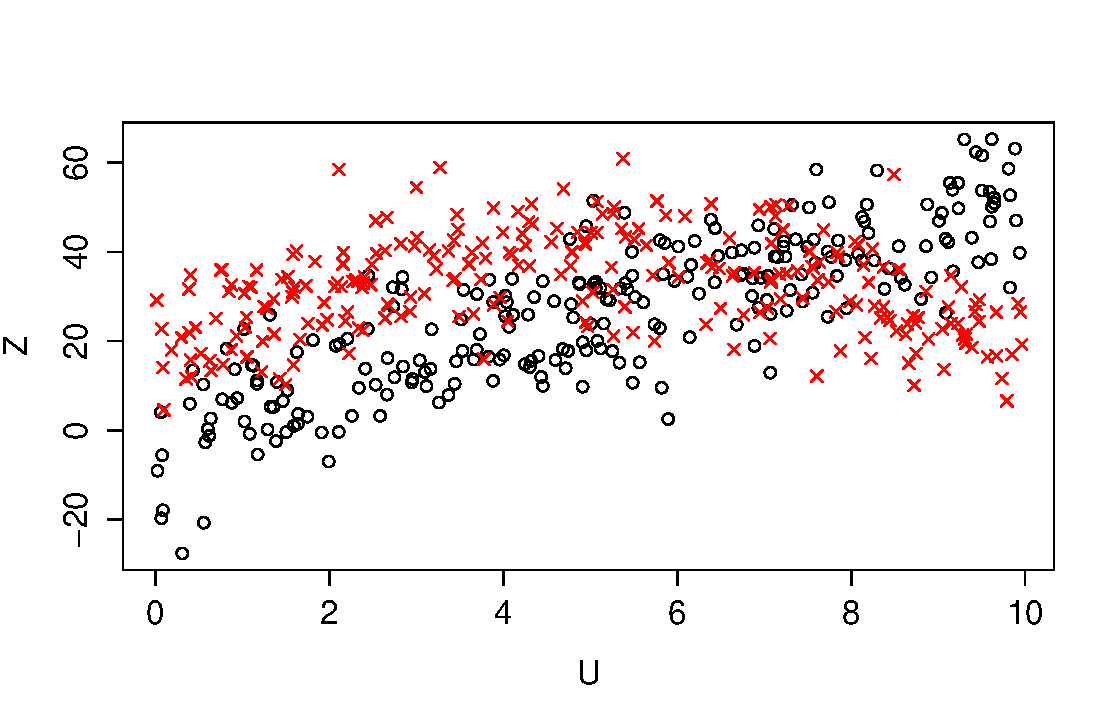
\includegraphics[width = .8\textwidth]{fig1.PDF}\\
\caption{Replication of Figure 1: "500 points drawn from the model: circles, points drawn from the first class, and crosses, points drawn from the second class". Note: The y-label in the published paper is Z, this should be R, since Z is a vector.} \label{f1}
\end{figure}

\clearpage
\begin{figure}[h!]
\centering
\begin{subfigure}[t]{.6\textwidth}
\caption{$\beta_{2}(1)$}
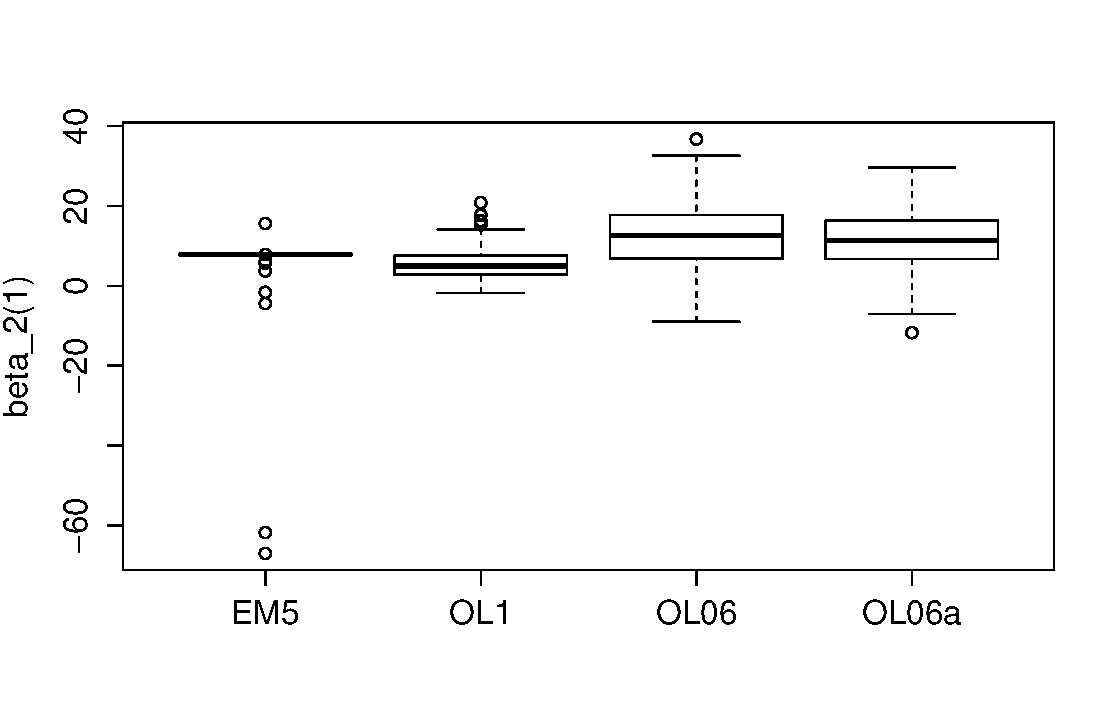
\includegraphics[width = \textwidth]{fig2_beta1.PDF}
\end{subfigure}
\begin{subfigure}[t]{.6\textwidth}
\caption{$\beta_{2}(2)$}
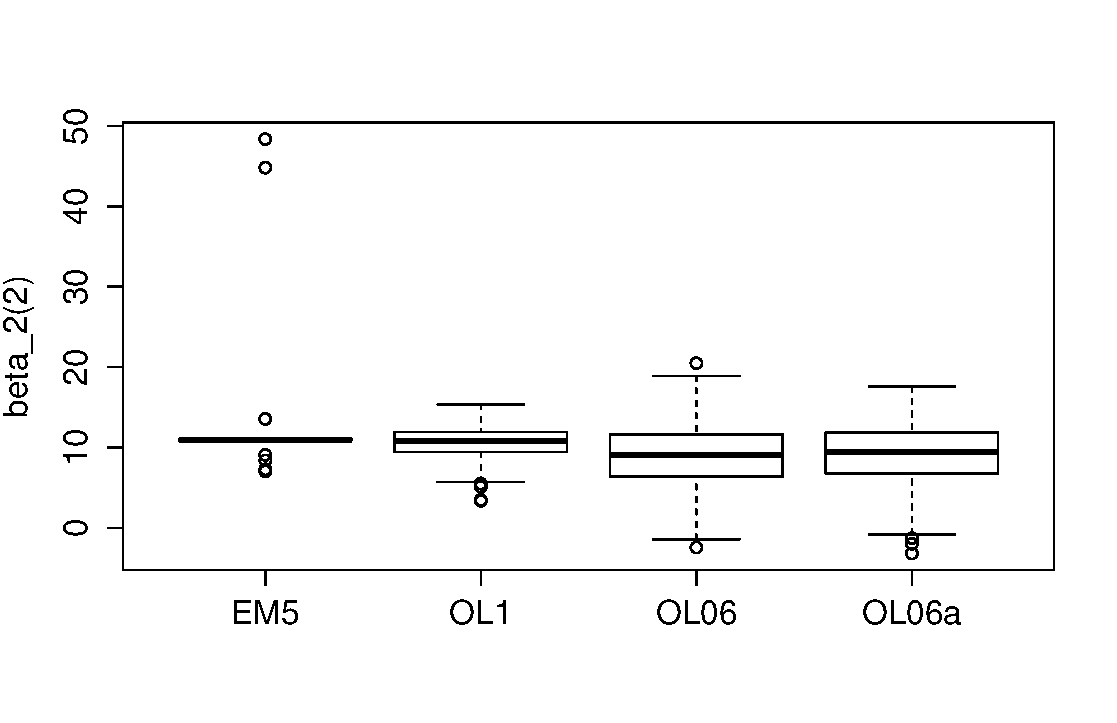
\includegraphics[width = \textwidth]{fig2_beta2.PDF}
\end{subfigure}
\begin{subfigure}[t]{.6\textwidth}
\caption{$\beta_{2}(3)$}
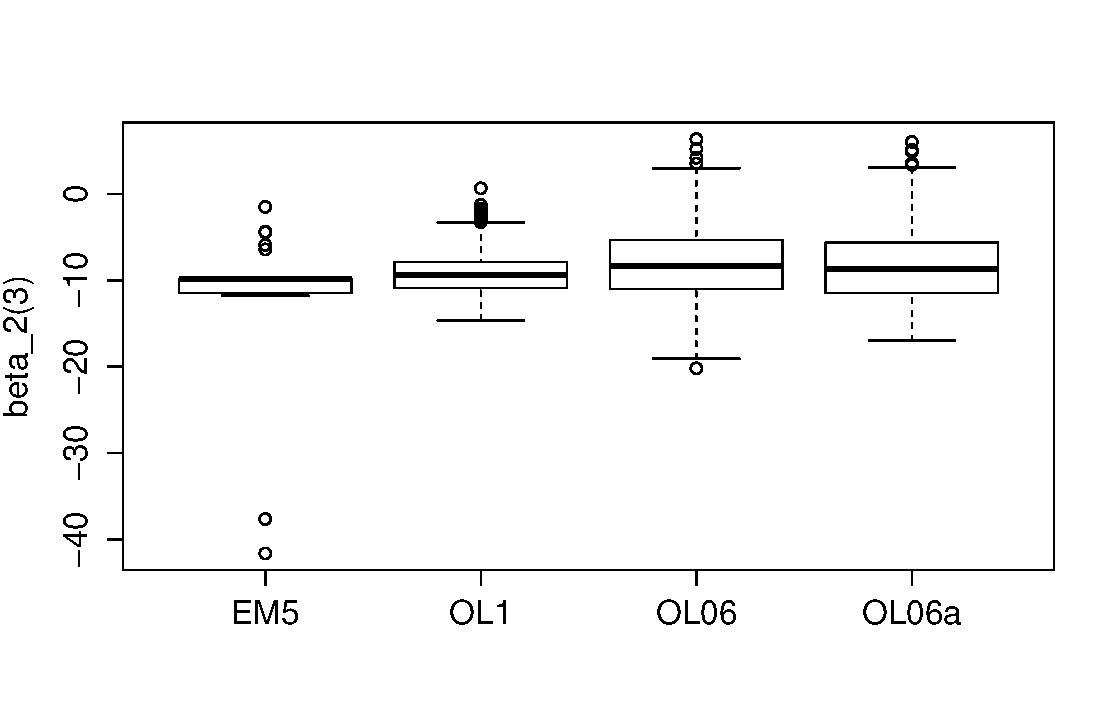
\includegraphics[width = \textwidth]{fig2_beta3.PDF}
\end{subfigure}
\caption{Replication of Figure 2: "Box-and-whisker plots of the three components of $\beta_{2}$, estimated from 500 independent runs of length $n = 100$", from left to right (batch EM, online EM  with $\gamma_{i} = 1/i$ (OL1), online EM with $\gamma_{i} = 1/i^{0.6}$ (OL06), and online EM with $\gamma_{i} = 1/i^{0.6}$(OL06a) with averaging starting from the 50th iteration} \label{f2}
\end{figure}

\clearpage
\begin{figure}[h!]
\centering
\begin{subfigure}[t]{.6\textwidth}
\caption{$\beta_{2}(1)$}
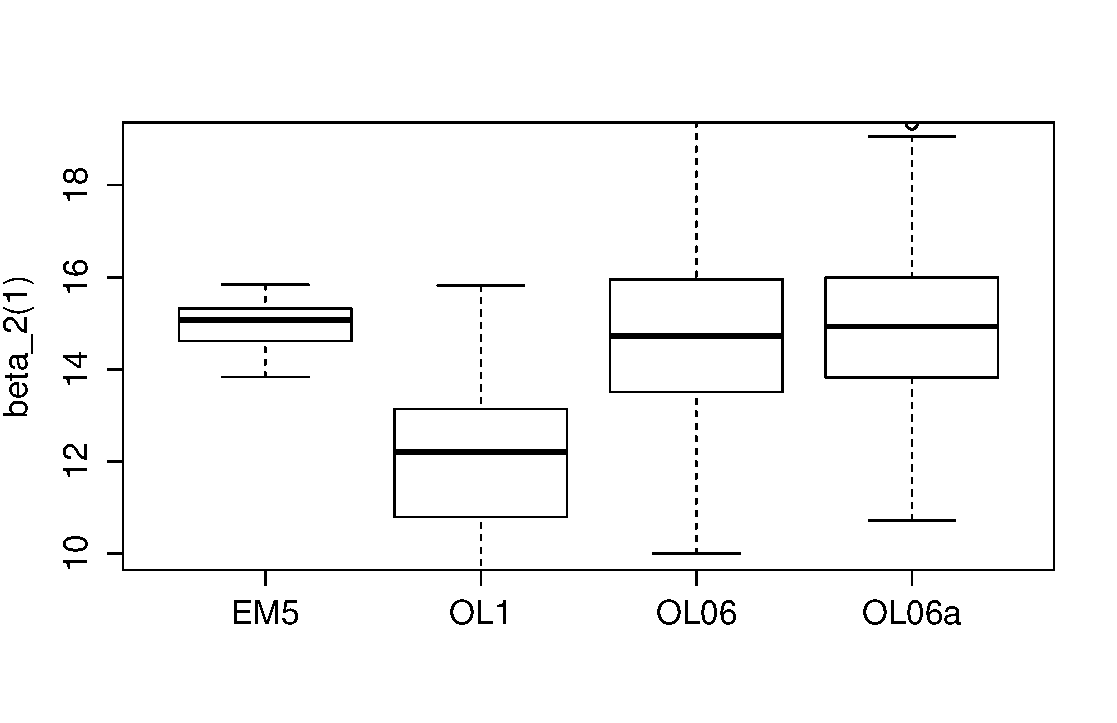
\includegraphics[width = \textwidth]{fig3_beta1.PDF}
\end{subfigure}
\begin{subfigure}[t]{.6\textwidth}
\caption{$\beta_{2}(2)$}
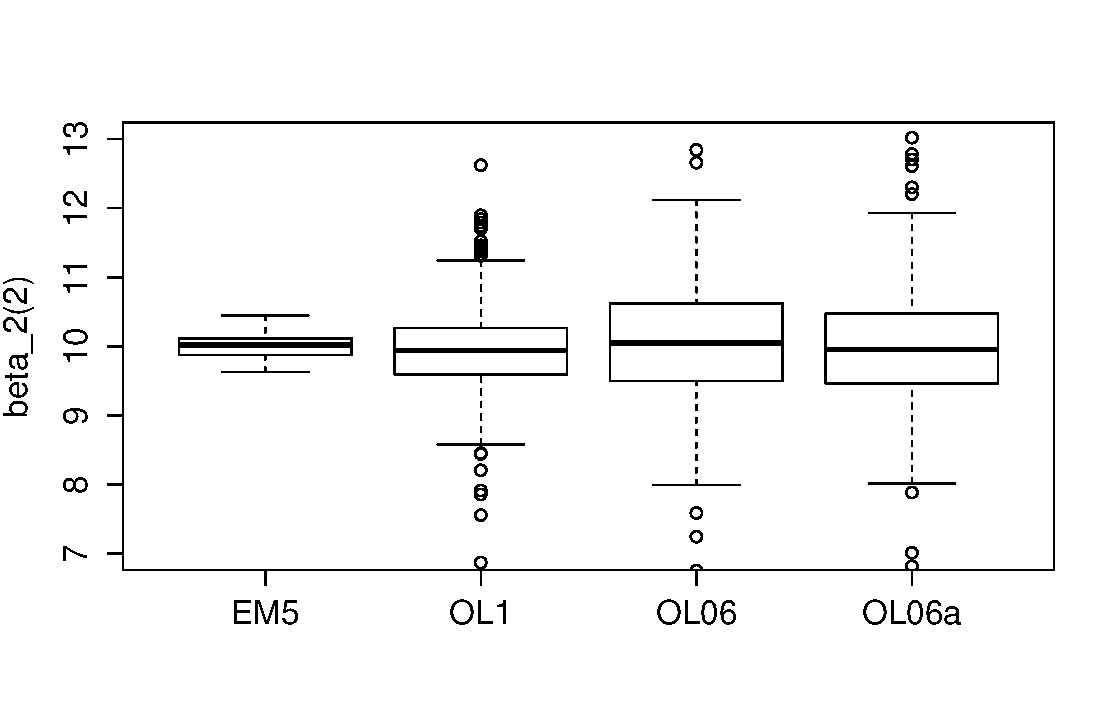
\includegraphics[width = \textwidth]{fig3_beta2.PDF}
\end{subfigure}
\begin{subfigure}[t]{.6\textwidth}
\caption{$\beta_{2}(3)$}
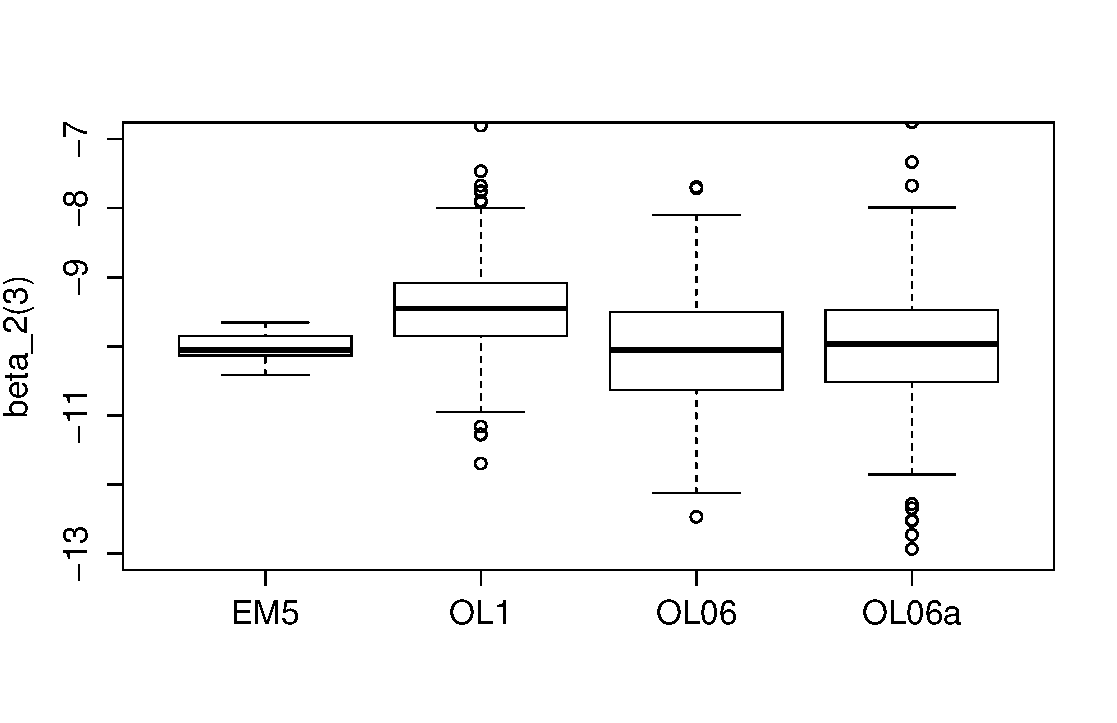
\includegraphics[width = \textwidth]{fig3_beta3.PDF}
\end{subfigure}
\caption{Replication of Figure 3: "Same plots as in Figure 2 for signals of length $n = 10,000$". In our analysis 500 runs of online EM were made, but only 50 runs of batch EM were made. } 
\end{figure}


\clearpage
\begin{figure}[h!]
\centering
\begin{subfigure}[t]{.6\textwidth}
\caption{$\beta_{2}(1)$}
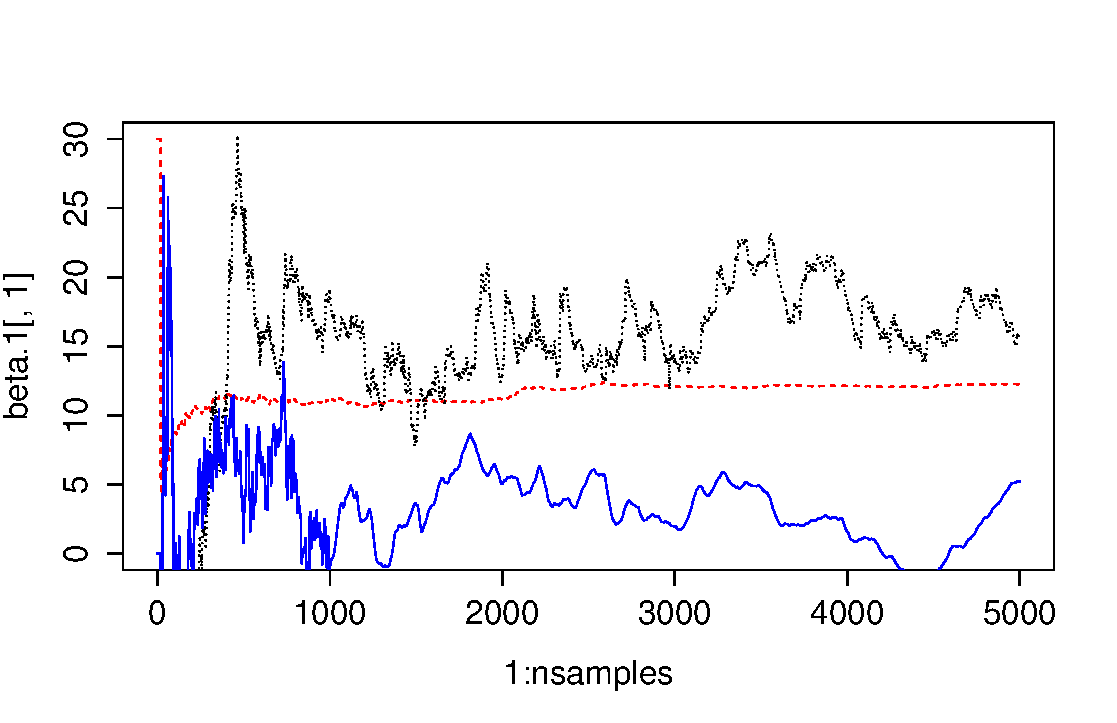
\includegraphics[width = \textwidth]{fig4_beta1.PDF}
\end{subfigure}
\begin{subfigure}[t]{.6\textwidth}
\caption{$\beta_{2}(2)$}
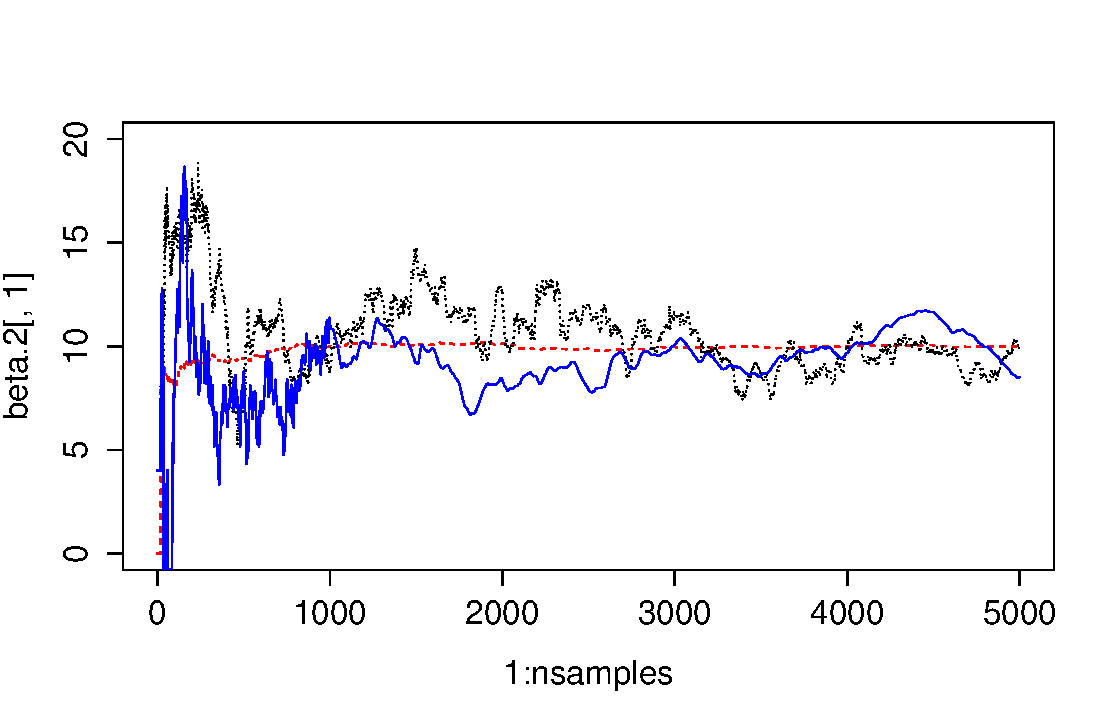
\includegraphics[width = \textwidth]{fig4_beta2.PDF}
\end{subfigure}
\begin{subfigure}[t]{.6\textwidth}
\caption{$\beta_{2}(3)$}
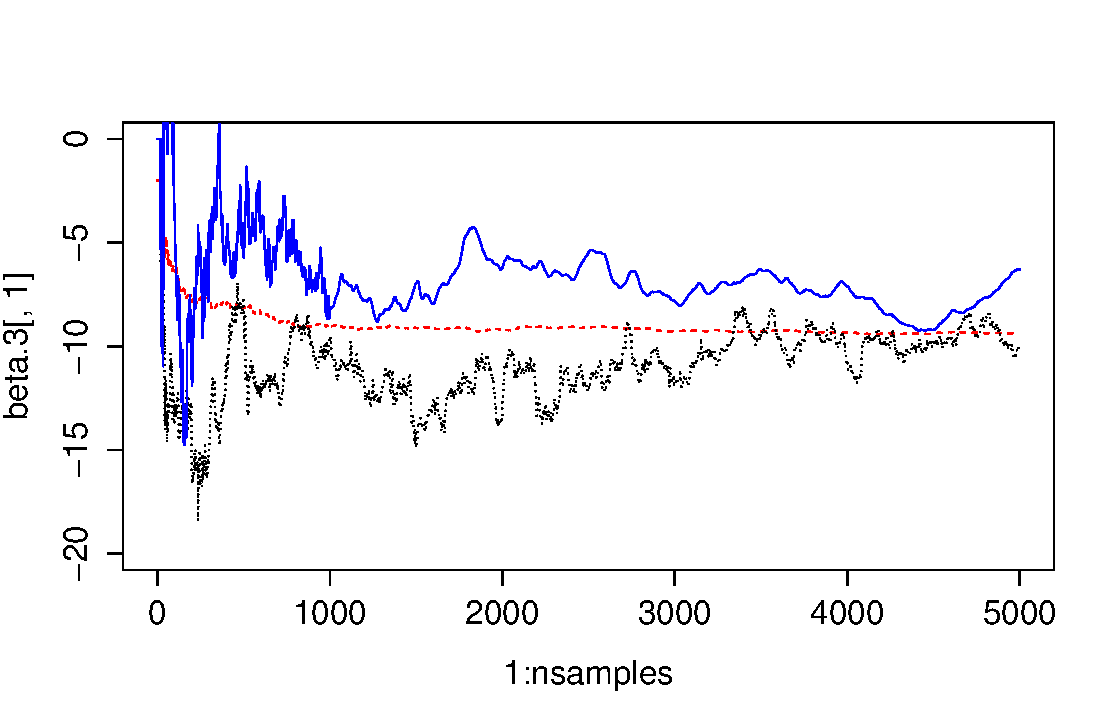
\includegraphics[width = \textwidth]{fig4_beta3.PDF}
\end{subfigure}
\caption{Replication of Figure 4: "Examples of parameters trajectories for the three components of $\beta_{2}$ for a signal length of n = 5,000: OL01, dashed line, OL06 dotted line, OL06a solid line (with averaging started after 1000 iterations)"} \label{f2}
\end{figure}

\clearpage
The boxplots for online EM largely match the boxplots in the paper. However, the batch EM boxplots tend to be narrower. This could likely have been caused by selecting initial values that were more similar to the true parameters than in the paper. Most of the replicated trajectories are nearly the same as those in the paper; however a few differ. This is, again, likely an artifact of the choice of intial values. Starting certain parameters in very different places than was done in the paper could cause different paths to be taken.  



\subsection{Novelty}
In this section, we apply the online EM method presented by Cappe and Moulines to the network traffic model proposed by Cao et al. However, applying online EM directly to this problem is not feasible, because the goal of the network model analysis is to try and determine changes in the mean overtime of  the number of messages going to and from the various router combinations.  Since at each time point, there is only one count of incoming and outgoing messages, there is only one data point for each time period. In the work of Cao et al., each data point is combined with its surrounding data points to give a window of 15 points to estimate the mean for each window using EM. Online EM only makes one pass through the data, so in this case each time period's means would be estimated with only 15 iterations of the algorithm, which is simply not enough to reach convergence at all consistently.\\

So, instead, we augment the data in each window. We split the original dataset into 26 windows, and found the mean and variance for each of the 16 origin-destination pairs (OD), i.e. corp $\rightarrow$ fddi, in each window. Then for each window, we drew 500 truncated multivariate normals, with a mean vector of observed sample means and a covariance matrix formed with the observed sample variances on the diagonal and zeros everywhere else. Then, we summed the appropriate OD pairs to get our "observed" link measurements. This preserves the latent influence of the unobserved OD pairs on the observed link measurements. Using this new "data", we then apply the online EM approach posed by Cappe and Moulines to each window. Specifically, we iterated between finding the sufficient statistics $m_{t}$ and $R^{(k)}$ using only the data point from the current iteration and maximizing $Q(\theta | \theta^{(t)})$ where $m_{t}$ and $R^{(k)}$ and  $Q(\theta | \theta^{(t)})$ are as given in the work of Cao et al. To display, these results, we build time series of the Poisson means overtime  for each path in the network (see Figure 5) and compare them to the time series obtained for batch EM as described by Cao et a. (see Figure 6). Both sets of time series are quite similar, suggesting online EM with the augmented data worked sufficiently well. \\

\begin{figure}[b!]
\centering
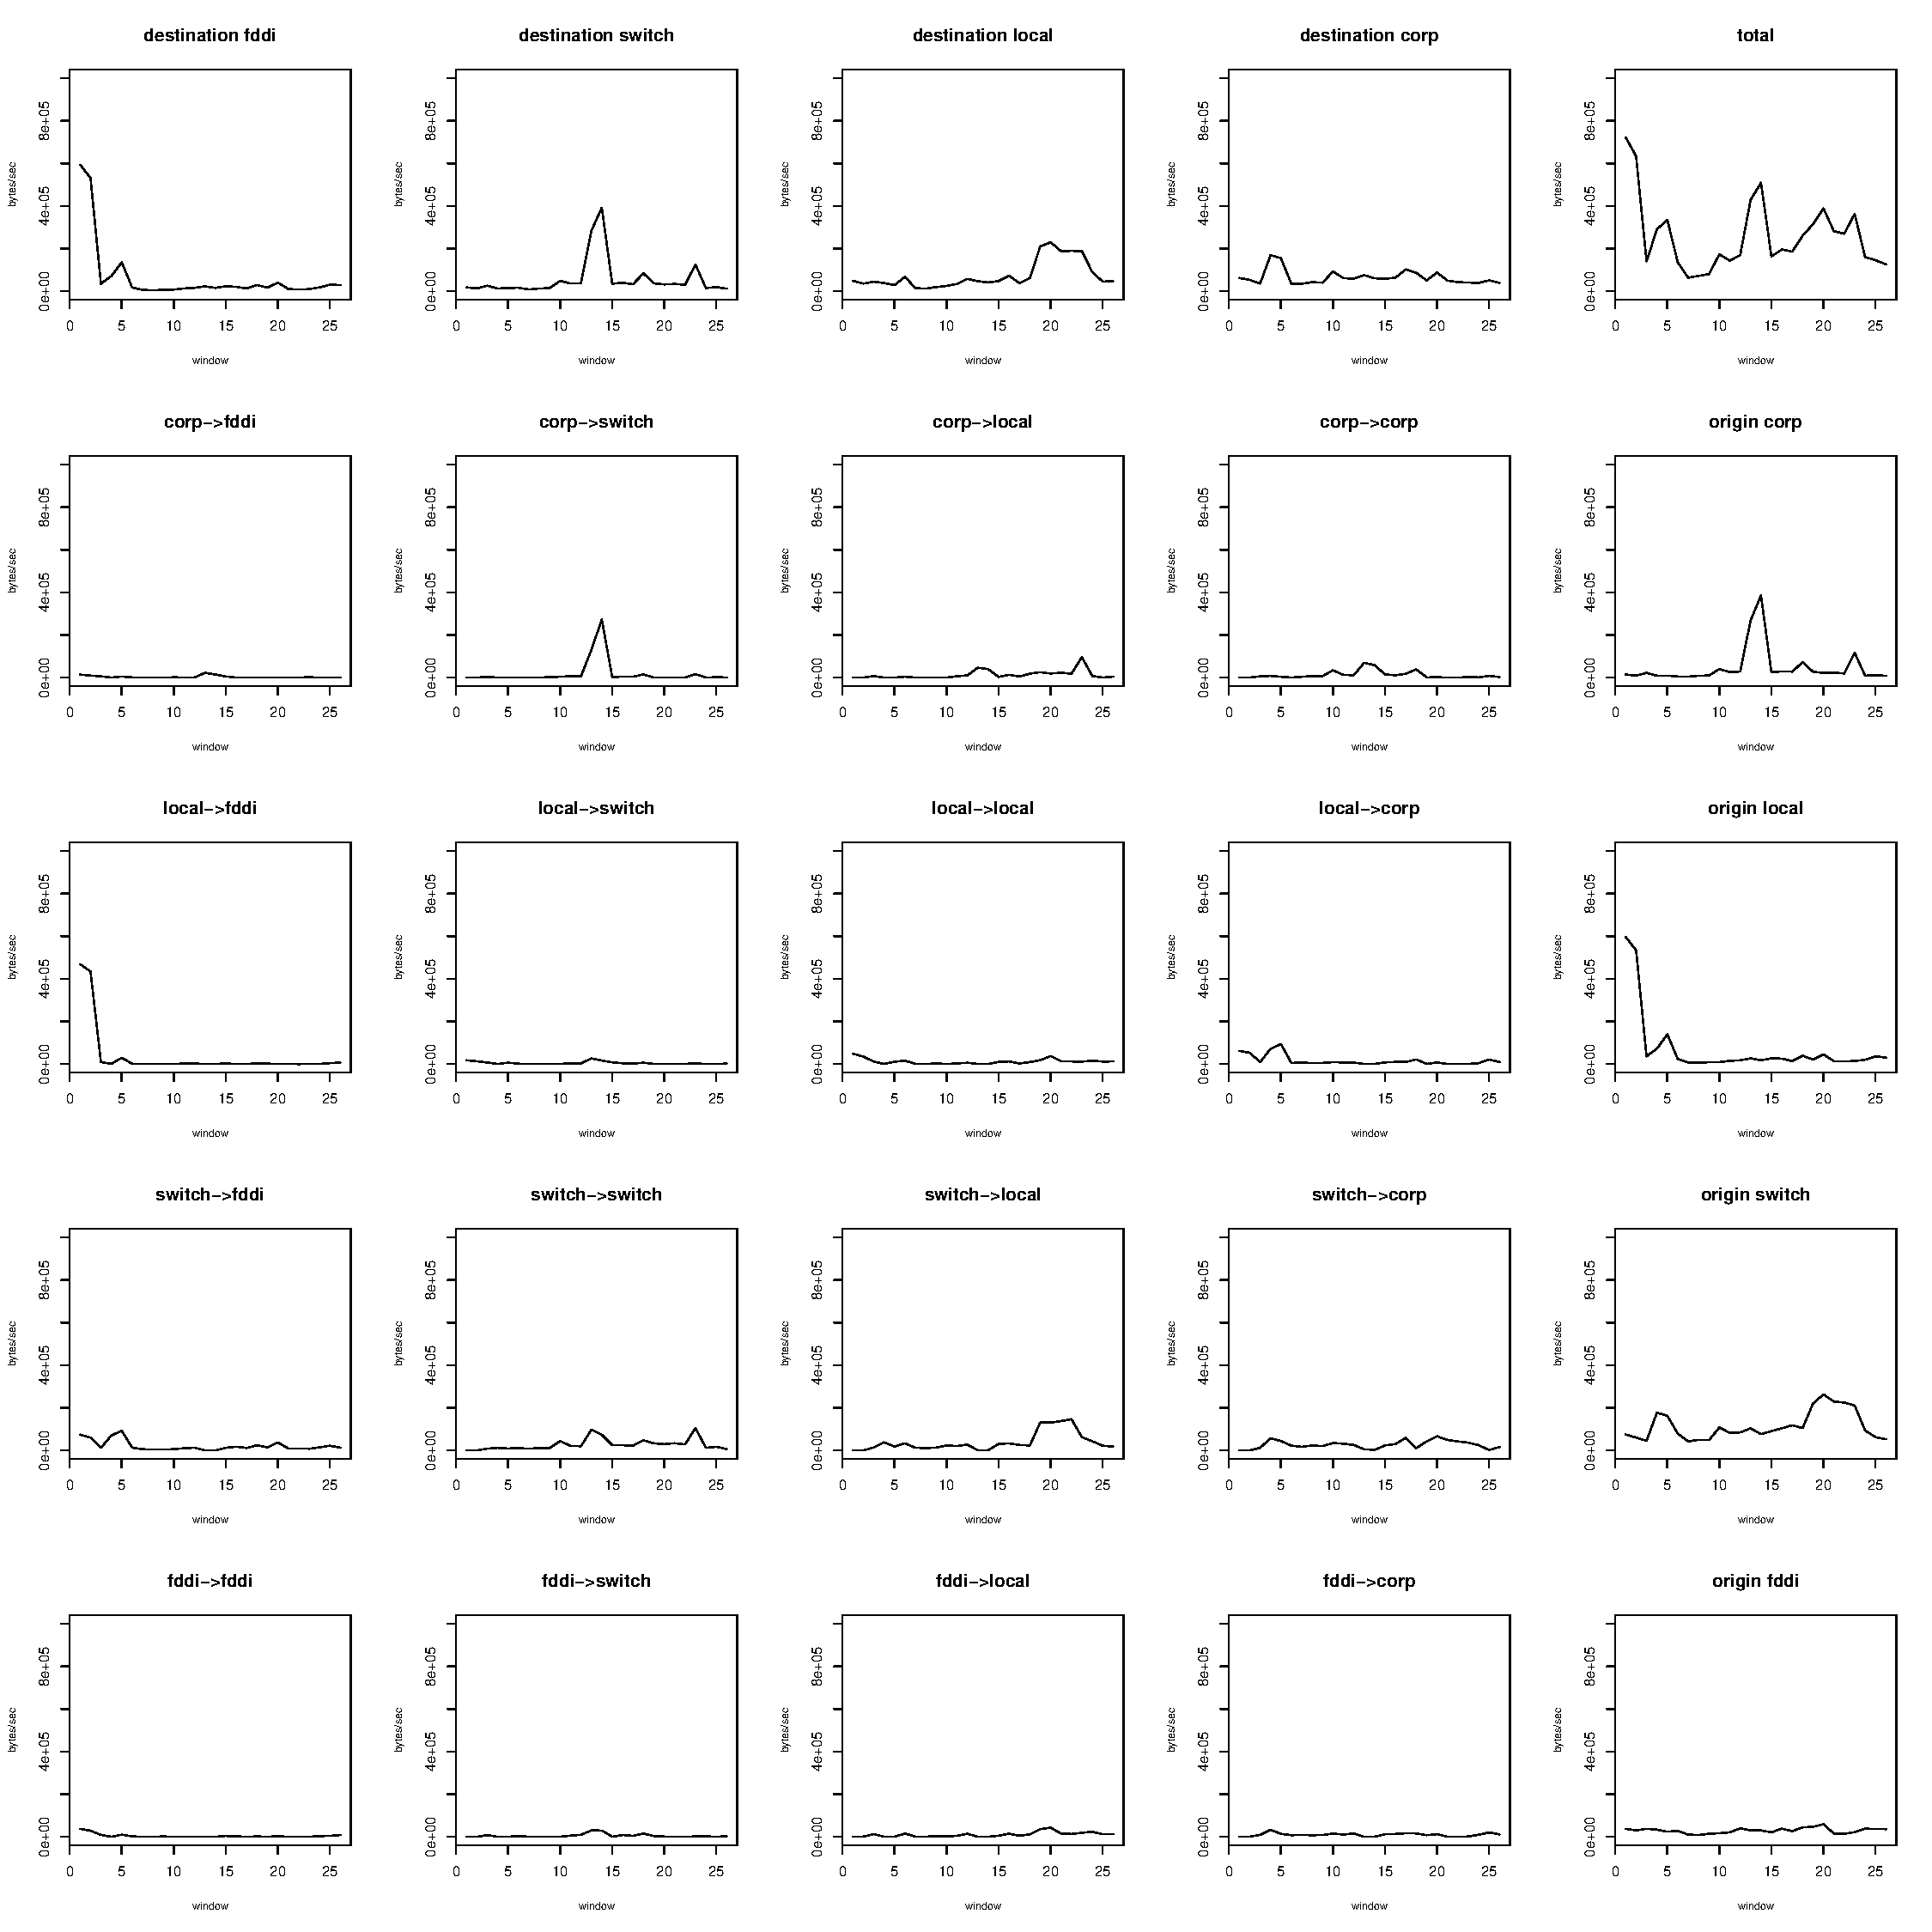
\includegraphics[width = \textwidth]{novelty_online_em.PDF}
\caption{This figure shows the time series obtained using our augmented online EM method. The graphs are quite similar to those obtained using batch EM.} \label{f2}
\end{figure}


\begin{figure}[b!]
\centering
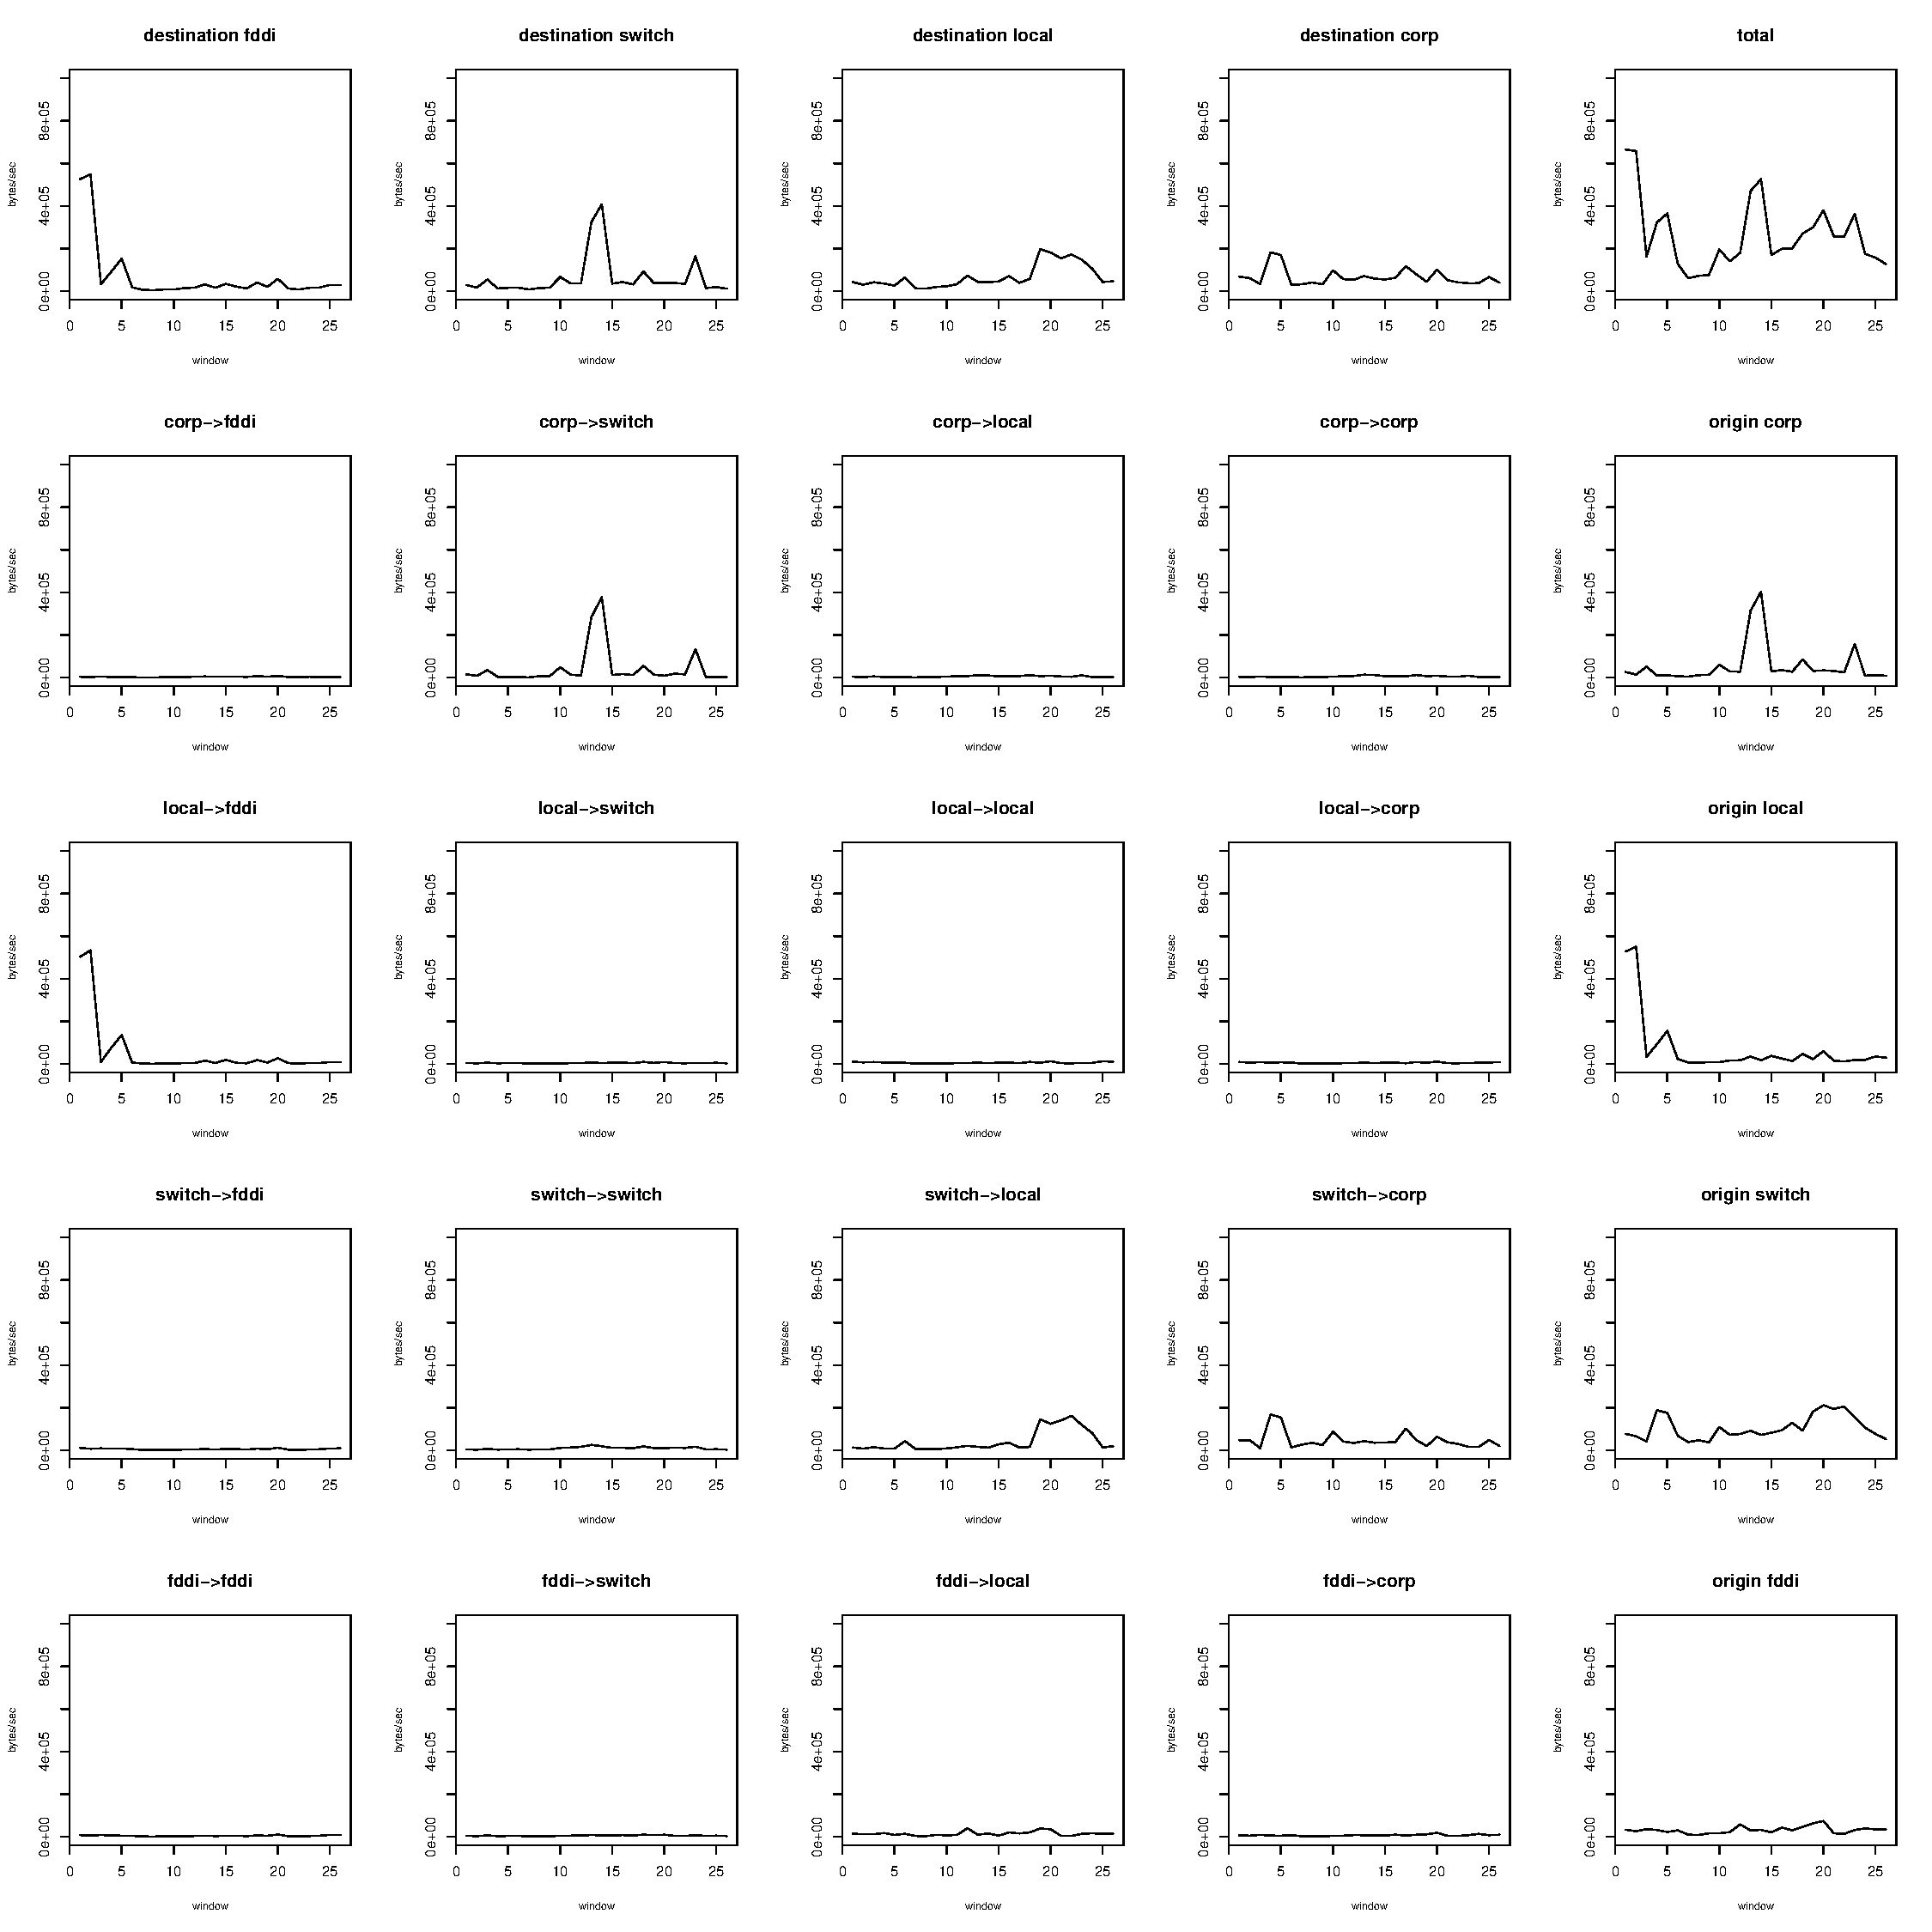
\includegraphics[width = 1\textwidth]{novelty_normal_em.PDF}\\
\caption{This figure shows the time series found in the network using the batch EM method given by Cao et al. It is included as a comparison.} \label{f2}
\end{figure}

From this analysis, we demonstrate that online EM is not appropriate for small data sets, since the algorithm is unlikely to converge. This work also suggests that applying a data augmentation strategy and then applying online EM may be a feasible way to work around small data sets that are converging very slowly with typical EM.  Nevertheless, significant theoretical work would need to be done to determine in what scenarios this method is appropriate and when such an approach is actually more efficient. 

\clearpage
\section{Conclusion}
The online EM approach proposed by Cappe and Moulines can be a useful and efficient alternative to traditional EM in certain cases. The approach is designed to solve problems that are both known to have latent variables and for which a traditional EM approach will break down. The most obvious example of this situation is for large data sets, since it becomes impossible to store and transfer all the data at once. In this situation, online EM is very useful in that it allows a practictioner to use only one data point at a time, rather than to work with all the data simultaneously.\\

Another situation where this online EM method is particularly useful is in cases where the true model of the data is unknown. Most online methods make use of the complete data information matrix of the model of the data. This does not present a theoretical problem when there is high confidence that the proposed model is correct. However, when the model is not correct, many of the theoretical gurantees given by other online methods are no longer valid. This makes the application of these models questionable. On the other hand, the online EM method proposed by Cappe and Moullines does not use the complete data information matrix. Thus, this method is likely to be much more robust to a misspecification of the model. \\

Despite these situations where the proposed online EM method is valuable, there are several cases where this approach breaks down. The most obvious of these cases is applying this method to relatively small data sets. In the proposed online method, there is only one pass through the data. This means that for small data sets, there are certainly not enough iterations through the algorithm to approach convergence, especially given that less information is being used on each iteration than is used in traditional batch EM. Thus, although applying the online EM algorithm may seem like an appealing option for overcoming a traditional EM implementation that is slow to convergene, for small data sets this approach is ill-advised. Instead, the algorithm will finish quickly, but convergence to the true maximum likelihood parameter estimates is unlikely to be obtained.\\

Another situation in which this approach does not perform well is for models where very little is know about the parameters a priori. In these cases, the online EM algorithm can easily break down because of poorly specified initial values. For example, in the Poisson mixture model, if little is know about the initial parameters, one might set all the Poisson means to be relatively low, even though the true means could be quite high. In such a case, if a particularly high data value is observed early in the implementation, the probability of observing such a value could be numerically zero, which causes the algorithm to break down. This issue can likely be overcome by implementing an "initialization period" where the first N data points would simply be collected and used to form initial paramter estimates. However, additional work will be needed to determine the best practices for doing this, such as determining the length of N in different scenarios and how much information loss occurs as a byproduct of using an initialization period. \\

In short, the online EM algorithm for latent data purported by Cappe and Moullines can be a valuable tool for more efficient implementation of the EM algorithm for large data sets. However, it should not be applied to small data sets and caution should be used when there is little prior information available about reasonable initial values for the parameters.

\end{document}

